% This is "sig-alternate.tex" V2.0 May 2012
% This file should be compiled with V2.5 of "sig-alternate.cls" May 2012
%
% This example file demonstrates the use of the 'sig-alternate.cls'
% V2.5 LaTeX2e document class file. It is for those submitting
% articles to ACM Conference Proceedings WHO DO NOT WISH TO
% STRICTLY ADHERE TO THE SIGS (PUBS-BOARD-ENDORSED) STYLE.
% The 'sig-alternate.cls' file will produce a similar-looking,
% albeit, 'tighter' paper resulting in, invariably, fewer pages.
%
% ----------------------------------------------------------------------------------------------------------------
% This .tex file (and associated .cls V2.5) produces:
%       1) The Permission Statement
%       2) The Conference (location) Info information
%       3) The Copyright Line with ACM data
%       4) NO page numbers
%
% as against the acm_proc_article-sp.cls file which
% DOES NOT produce 1) thru' 3) above.
%
% Using 'sig-alternate.cls' you have control, however, from within
% the source .tex file, over both the CopyrightYear
% (defaulted to 200X) and the ACM Copyright Data
% (defaulted to X-XXXXX-XX-X/XX/XX).
% e.g.
% \CopyrightYear{2007} will cause 2007 to appear in the copyright line.
% \crdata{0-12345-67-8/90/12} will cause 0-12345-67-8/90/12 to appear in the copyright line.
%
% ---------------------------------------------------------------------------------------------------------------
% This .tex source is an example which *does* use
% the .bib file (from which the .bbl file % is produced).
% REMEMBER HOWEVER: After having produced the .bbl file,
% and prior to final submission, you *NEED* to 'insert'
% your .bbl file into your source .tex file so as to provide
% ONE 'self-contained' source file.
%
% ================= IF YOU HAVE QUESTIONS =======================
% Questions regarding the SIGS styles, SIGS policies and
% procedures, Conferences etc. should be sent to
% Adrienne Griscti (griscti@acm.org)
%
% Technical questions _only_ to
% Gerald Murray (murray@hq.acm.org)
% ===============================================================
%
% For tracking purposes - this is V2.0 - May 2012

\documentclass{sig-alternate}
\usepackage{hyperref}
\usepackage{breakurl}
\usepackage{natbib} 

\makeatletter
\def\@copyrightspace{\relax}
\makeatother

\begin{document} \sloppy

%
% --- Author Metadata here ---
% \conferenceinfo{University of British Columbia}{Vancouver, BC, Canada}
% \CopyrightYear{2014} % Allows default copyright year (20XX) to be over-ridden - IF NEED BE.
% \crdata{}  % Allows default copyright data (0-89791-88-6/97/05) to be over-ridden - IF NEED BE.
% --- End of Author Metadata ---

\title{Plan/Proof-of-Concept: Game Development in Factor}
% \subtitle{[Extended Abstract]
% \titlenote{A full version of this paper is available as
% \textit{Author's Guide to Preparing ACM SIG Proceedings Using
% \LaTeX$2_\epsilon$\ and BibTeX} at
% \texttt{www.acm.org/eaddress.htm}}}
%
% You need the command \numberofauthors to handle the 'placement
% and alignment' of the authors beneath the title.
%
% For aesthetic reasons, we recommend 'three authors at a time'
% i.e. three 'name/affiliation blocks' be placed beneath the title.
%
% NOTE: You are NOT restricted in how many 'rows' of
% "name/affiliations" may appear. We just ask that you restrict
% the number of 'columns' to three.
%
% Because of the available 'opening page real-estate'
% we ask you to refrain from putting more than six authors
% (two rows with three columns) beneath the article title.
% More than six makes the first-page appear very cluttered indeed.
%
% Use the \alignauthor commands to handle the names
% and affiliations for an 'aesthetic maximum' of six authors.
% Add names, affiliations, addresses for
% the seventh etc. author(s) as the argument for the
% \additionalauthors command.
% These 'additional authors' will be output/set for you
% without further effort on your part as the last section in
% the body of your article BEFORE References or any Appendices.

\numberofauthors{5} %  in this sample file, there are a *total*
% of EIGHT authors. SIX appear on the 'first-page' (for formatting
% reasons) and the remaining two appear in the \additionalauthors section.
%
\author{
% You can go ahead and credit any number of authors here,
% e.g. one 'row of three' or two rows (consisting of one row of three
% and a second row of one, two or three).
%
% The command \alignauthor (no curly braces needed) should
% precede each author name, affiliation/snail-mail address and
% e-mail address. Additionally, tag each line of
% affiliation/address with \affaddr, and tag the
% e-mail address with \email.
%
% 1st. author
\alignauthor
Reggie Gillett\\
\affaddr{27133123}\\
\affaddr{w6k8}\\
\email{reggie.gillett@gmail.com}
% 2nd. author
\alignauthor
Graham St-Laurent\\
\affaddr{23310121}\\
\affaddr{i5l8}\\
\email{gstlaurent@gmail.com}
% 3rd. author
\alignauthor Lynsey Haynes\\
\affaddr{12686119}\\
\affaddr{a4h8}\\
\email{lynseyahaynes@gmail.com}
\and  % use '\and' if you need 'another row' of author names
% 4th. author
\alignauthor Brittany Roesch\\
\affaddr{22015119}\\
\affaddr{r1d8}\\
\email{brroesch@gmail.com}
% 5th. author
\alignauthor Gord Minaker\\
\affaddr{34615112}\\
\affaddr{u4s8}\\
\email{gordonminaker@hotmail.com}
}
% % There's nothing stopping you putting the seventh, eighth, etc.
% % author on the opening page (as the 'third row') but we ask,
% % for aesthetic reasons that you place these 'additional authors'
% % in the \additional authors block, viz.
% \additionalauthors{Additional authors: John Smith (The Th{\o}rv{\"a}ld Group,
% email: {\texttt{jsmith@affiliation.org}}) and Julius P.~Kumquat
% (The Kumquat Consortium, email: {\texttt{jpkumquat@consortium.net}}).}
% \date{30 July 1999}
% Just remember to make sure that the TOTAL number of authors
% is the number that will appear on the first page PLUS the
% number that will appear in the \additionalauthors section.

\maketitle
\begin{abstract}
This paper outlines the implementation of components and tools necessary to create a substantial program in Factor. In the context of this paper, discussions are based around the development of an interactive game. The authors discuss the implementation behind graphical user interfaces components including user input and output. In addition, we discuss some components of the Factor language that are integral to development including the object system, unit testing and debugging.
\end{abstract}

% % A category with the (minimum) three required fields
% \category{H.4}{Information Systems Applications}{Miscellaneous}
% %A category including the fourth, optional field follows...
\category{D.3.3}{Programming Languages}{Language Constructs and Features}

\terms{Languages}

\keywords{Factor, Game, stack-based languages, concatenative languages}

\section{Introduction} 
For our end-of-term project, we have outlined a plan to create a substantial program in a stack-based language called Factor. Previously we have researched the tools and features in the language, and discussed the implications of programming in a concatenative language. The current paper expands on our previous investigations into the language and discusses how we plan to use Factor to accomplish the development of our game. Along the way we will highlight the components required for our implementation, provide example code behind our implementation, and provide screenshots of our game output. 

\section{Game Overview}
\subsection{Game Design}
In our game, the player will be presented with a collection of hamburger ingredients, a collection of actions, and a goal hamburger. It is the player's task to apply the various actions to the ingredients in an appropriate order to produce the goal hamburger, and there can be more than one way of doing it. The catch: the ingredients are presented in a regular Last-In-First-Out stack, and the actions can, correspondingly, only be applied to the topmost elements of the stack. Initially, our game will only consist of one level, with a small collection of ingredients and a small selection of actions, but the complete game would consist of increasingly complex levels gradually introducing a large variety of actions and ingredients, not all of which would necessarily be available in each level. To tie it all together and provide further enjoyment for the player, the game will provide context for each level with an overarching story about working in a (somewhat surreal) restaurant.

\subsection{Game Layout and Example}
\begin{figure}[h!]
  \centering
    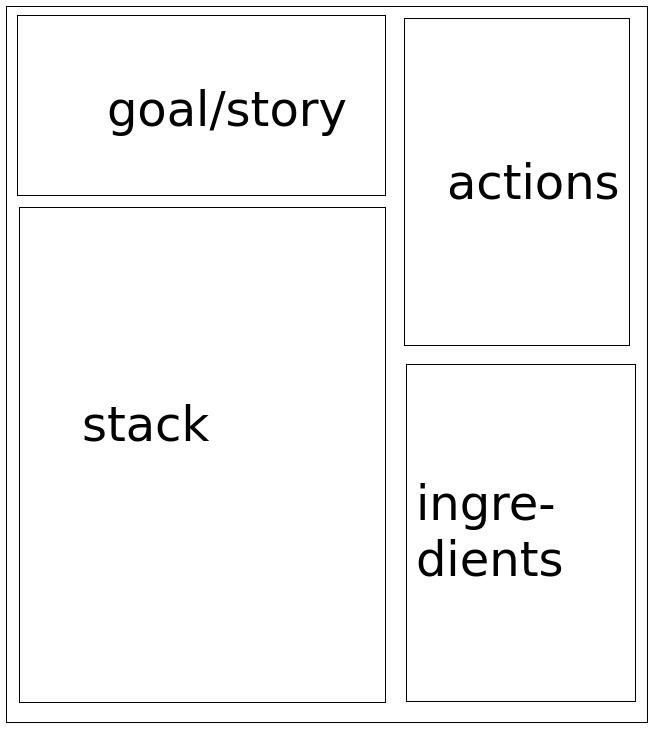
\includegraphics[scale=.3]{layout.jpeg}
  \caption{The window layout.}
  \label{fig:layout}
\end{figure}

Figure~\ref{fig:layout} shows the layout for a typical game level. Each component is described below:
\begin{itemize}
\item \textbf{goal/story}: some text describing the current scenario and the player's current goal.
\\
\textit{Example: The customer wants a plain hamburger. Build one and send it.}
\item \textbf{stack}: a graphical representation of the current state of the stack.
\\
\textit{Example: From the bottom up, images of the bottom half of a bun, the top half of a bun, and a raw patty.}
\item \textbf{actions}: a group of buttons representing the available actions. Each button will have a name (the name of the action), and a description of its effect.
\\
\textit{Example: Swap (switches order of the top two items), Cook (remove the top element of the stack and replace it with a cooked version of it), Squish (takes all elements in the stack and compresses them together into a compact sandwich), Send to Customer (Removes the top element from the stack and submits it to the customer).}
\item \textbf{ingredients}: In levels where the player is able to push and pop elements to and from the stack, this area represents a bag of unordered ingredients. Each ingredient is a button that, when clicked, will push its ingredient to the stack.
\\
\textit{Example: In a level with optional pickles, there could be a pickle here. In our first level, there will be no extra ingredients.}
\end{itemize}

Taking as a starting point the level described in the above examples, the player could complete it by pressing, in order Cook, Swap, Squish, and Send to Customer. If the player presses Cook while there is a bun on the stack, though, it will be burnt, the customer will not be satisfied, and the player will lose. If the player presses Squish without the ingredients in the proper order, something disgusting is the result, and once again, the customer will not be satisfied and the player will lose. On the other hand, if the player follows the solution sequence but with a couple of extra swaps (Cook, Swap, Swap, Swap, Squish, Send), this will still be a valid solution and the player will win. If this swap-happy player decides to press swap one more time before Send, though, we will get a stack underflow. In order to replicate the misery of this situaion in our game without forcing an immediate loss, any stack underflow does nothing but provide an insulting message for the player.

\section{Object Orientedness}
Our game will be using Factor`s implementation of objects to represent different elements that can be pushed onto the stack. An understanding of Factor's OO syntax and behaviour will be beneficial moving forward with implmentation of our game. Although technically all variables are objects in factor, we are looking at specifically those with multiple slots, called Tuples\cite{OOTuples}. Declaring a tuple with slots in Factor is similar to creating a new class in Java with fields. In the example below, an object called `element` with slots x, y, proper, and object would look like: 
\begin{verbatim}
TUPLE: burger x y proper object ;
\end{verbatim}
A basic constructor of an element could look like:

\begin{verbatim}
: <burger> ( -- burger )
burger new ;
\end{verbatim}

This constructor creates a new element with empty fields. Fields can be set and read by the set and get methods. Setting the field x would look like:

\begin{verbatim}
>>x
\end{verbatim}

while getting the value of field x would look like

\begin{verbatim}
x>>
\end{verbatim}

A more complicated constructor might use a combination of the set methods above, or use the BOA\cite{boa} (By Order of Arguments) constructor. It creates the specified tuple by grabbing its required number of fields off of the data stack. A BOA constructor that we might use in our game: 

\begin{verbatim}
: <burger> ( x y object -- burger )
 -1 swap burger boa ;
\end{verbatim}

The tuple constructed then looks like :

\begin{verbatim}
T{burger {x 0} {y 0} {proper -1} {object [+]}}
\end{verbatim}

\section{User Interface}
Central to any game is some form of user interface. The player should have some graphical interface presented to them that they can interact with. A trivial implementation of this would be a simple command-line interface. However, for our game we want a more of a challenge and in turn, a better learning opportunity. We will create windows which respond to user input and display graphics.

UI elements in factor are implemented using \textit{gadgets}.  Factor's documentation describes them as: ``graphical elements which respond to user input"  \cite{BuildingUI}. It goes on to give a more technical description, ``gadgets are tuples which (directly or indirectly) inherit from the class \texttt{gadget}"\cite{BuildingUI}. Factor's creators provide us will a multitude of pre-made gadgets, with the ability to extend or create or own. Gadgets are key to displaying windows within a user's operating system and we will be using them extensively in our discussion of creating a user interface.
\begin{verbatim}
: make-window ( -- )
    <pane>
    "Gadget!"
    open-window
\end{verbatim}

The above is a word definition which creates a trivial pane. A \textit{pane} is one of the pre-made gadgets factor provides for displaying formatted text \cite{Pane}.  Factor provides a word, texttt{open-window}, that places a gadget in a new window. It takes a gadget and a string as its arguments, the string functioning as the window's title. We can see in the code above, we call the word that constructs a new pane: \texttt{<pane>} (this creates a pane and puts it on the stack). We then put the string ``Gadget!" on the stack. We subsequently call open-window which consumes these two elements and produces a window with an empty pane and the title ``Gadget!''. Essentially, this gets us a titled window with no formatting and no content. For our implementation of our game, we need to be able to make and change the content of pane and preferably we should be able to set some parameters of the window, particularly its size.  We can do both of these things by extending our previous code as follows:
\begin{verbatim}
: make-window ( -- )
    <pane>
    dup
    T{ world-attributes { title "Gadget!" }
        { pref-dim { 250 50 } } }
    open-window
    [  "This is an example of a Gadget." print ]
    with-pane
    \end{verbatim}

Instead of simply passing a string to open-window we now pass a \texttt{world-attributes} tuple. This controls the attributes of the window that is being opened. This allows us to set the window's initial dimensions, title and a slew of other properties \cite{world}.   For the sake of simplicity, in this case we have simply designated a title and preferred dimensions.  You will notice that we have also duplicated our pane. This will be handy when we want to add some content to it.

\begin{figure}[h!]
  \centering
    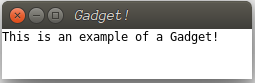
\includegraphics[scale=.7]{Gadget.png}
  \caption{A simple window.}
  \label{fig:gadget}
\end{figure}

Each pane has a pane-stream which handles output and displays it on the associated pane rather than the standard output \cite{Pane}. Factor provides several ways of manipulating this stream. The one we use above is \texttt{with-pane}. This word takes a pane and a quotation, clears the pane and calls the quotation replacing its output stream with that of the pane \cite{withpane}. In our example this quotation simply prints the phrase ``This is an example of a gadget".  Calling this word gives us the window illustrated in Figure~\ref{fig:gadget}.

Gadgets can have multiple child gadgets which are displayed within them. The window itself is in fact a \textit{World}, which is a type of gadget. The World acts as the root of a tree which in our example only contains one child, our pane. This tree structure allows for a heirarchical scheme that facilitates more complex window arrangements.

\subsection{Key Commands}

At some point, our game will have to receive and respond to input from the player. In most games, including ours, this takes the form of responding to key strokes or mouse clicks. In Factor terminology, user actions, including mouse clicks and keystrokes, are referred to as \textit{gestures}. Factor conveniently provides us with a fairly simple word to implement responses to gestures in the Gadget environment: \texttt{set-gestures}. This takes a class and a hashtable as arguments. The hashtable maps gestures to quotations with a stack effect in the context of the given class\cite{setgestures}. The gestures are represented as tuples. We can add this to our previously created window as follows:

\begin{verbatim}
: make-window ( -- )
    <pane>
    dup
    T{ world-attributes { title "Gadget!" }
        { pref-dim { 250 50 } } }
    open-window*
    swap
    [  "This is an example of a Gadget." print ]
    with-pane
    class-of
    H{
     { T{ key-down f f "UP" } 
       [ gadget-child [ "Up" print ] with-pane ] }
       T{ key-down f f "DOWN" } 
       [ gadget-child [ "Down" print ] with-pane ] }
       T{ key-down f f "LEFT" } 
       [ gadget-child [ "Left" print ] with-pane ] }
       T{ key-down f f " " } 
       [ gadget-child [ "Right" print ] with-pane ] }
	 }
    set-gestures
    \end{verbatim}
    
You'll notice that the call to \texttt{open-window} is now suffixed with an asterisk. This is an alternate word with the same functionality that returns the window that is created to the stack. We use it here to allow for more concise code. We then get its class using \texttt{class-of} and pass this and a hashtable containing several mappings for the direction keys. The details of the quotation are unimportant to our discussion, however the effect is printing the name of the key that was pressed in the window we have created.

\subsection{Buttons}

Buttons are another method of handling user input. In Factor, buttons are gadgets. Therefore they can be added to any existing gadget. The following code adds a button to our previously created interface (the gestures and text we added in the previous section have been removed for clarity):

\begin{verbatim}
: make-window ( -- )
    <pane>
    dup
    T{ world-attributes { title "Gadget!" }
        { pref-dim { 250 50 } } }
    open-window
    <pane-stream>
    "Click me!" [ "Clicked!" print ] <border-button>
    swap
    write-gadget
    \end{verbatim}

There are a few things that we do slightly differently in order to add a button. In this case we duplicate the pane we created initially. This is solely so that later in the word's execution we can attain an explicit reference to its output stream: the call to \texttt{<pane-stream>}. You will notice that we have also reverted to \texttt{open-window} without the asterisk, as in this illustrative example we no longer need the window on the stack. We create a button using the constructor \texttt{<border-button>}, which takes a string and a quotation as arguments. Factor provides several styles of button with associated constructors, for this example we use \texttt{<border-button>} which produces a standard button with a border \cite{button}. We then do a swap-a-roo and call \texttt{write-gadget} which places a gadget in an output stream, in this case, the pane-stream we stored on the stack earlier.


\subsection{Image Rendering}
The final component of our UI will be the actual visual environment: images. Factor provides several different methods to do this. One way is to use the built-in OpenGL bindings to dynamically generate images. This is done by creating a new gadget to use as the canvas, and then using words from the \texttt{opengl} vocabulary to render the image. For instance, here is some code that will generate a red rectangle (rendered in Figure 3):
\begin{verbatim}
    20 20 1 glScalef    ! set 1:20 scale for XY                
    COLOR: red gl-color ! current colour = red  
    { 3 4 }  { 1 2 }  gl-fill-rect  
       ! rectangle at pos ( 3 4 ) of size ( 1 2 )
\end{verbatim}


\begin{figure}[h!]
  \centering
    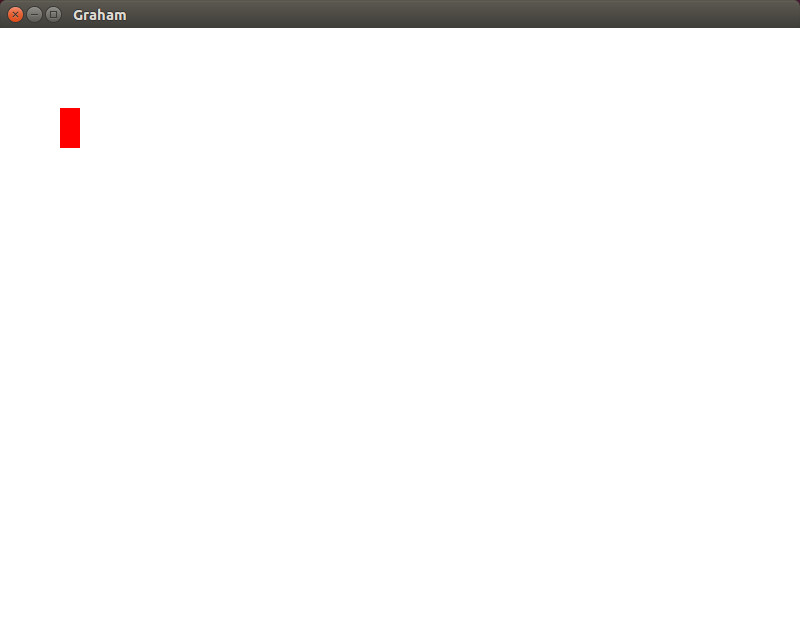
\includegraphics[scale=.3]{rectangle.jpg}
  \caption{A red rectangle.}
\end{figure}



This can be quite laborious, but luckily, there is an easier way: simply read and render image files. Factor provides support for creating, manipulating, and displaying images in dozens of different formats. When working with ready image files, this is most easily accomplished by using the \texttt{<image-gadget>} constructor, which takes a string with an image file pathname and produces an \texttt{image-gadget}. As its name suggests, an image gadget is simply a gadget that displays an image. Here's an example that stacks a series of hamburger-related images on top of each other using a \texttt{pile} layout gadget. Then it, alongside some text (\texttt{pane} gadgets) is added to the top-most \texttt{super-gadget}, which is initialized as a 600 by 900 pixel window. The pane gadgets in the example serve as placeholders for where other components could be be a more sophisticated program (Figure 4).


\begin{verbatim}
USING: kernel accessors ui ui.gadgets ui.render 
ui.gadgets.editors images.viewer combinators sequences
ui.gadgets.packs ui.gadgets.panes ;
IN: cs311

TUPLE: super-gadget < gadget ;
: <super-gadget> ( -- gg ) super-gadget new ;

M: super-gadget pref-dim* ( gadget -- {xy} ) 
    drop { 600 900 } ;


: burgerpic ( -- )
    <super-gadget>
    <shelf>

    <pile>
    <pane> dup { 200 200 } >>pref-dim
    [ "This is where some writing could go.
       Perhaps some instructions?." write ] with-pane
    add-gadget

    { "~/coolimages/topbun.png"
      "~/coolimages/grilledpatty.png"
      "~/coolimages/rawpatty.png"
      "~/coolimages/bottombun.png"
      "~/coolimages/burger.png" }
    [ <image-gadget> add-gadget ] each
    add-gadget

    <pane> dup { 200 400 } >>pref-dim
    [ """
This is where the buttons will go.

Later levels will have lots of buttons.

But since we probably won't implement
many levels, there might not be
much to see here.

The end.
""" write ] with-pane
    add-gadget
    add-gadget "Hamburger" open-window ;
\end{verbatim}

\begin{figure}[h!]
  \centering
    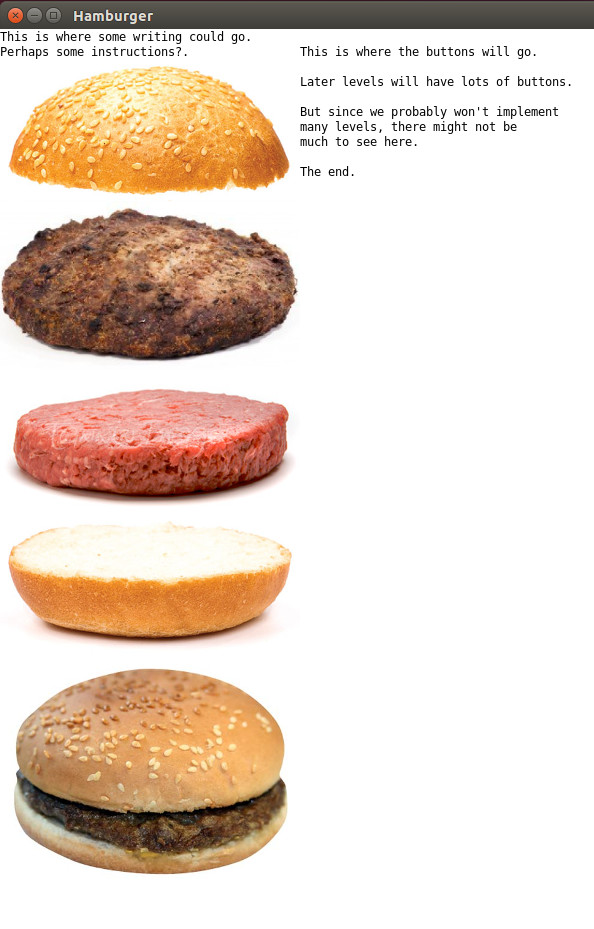
\includegraphics[scale=.35]{image-gadget.jpg}
  \caption{A gadget full of images.}
\end{figure}


\section{Testing}
Unit testing is important to consider in the small, initial stages of development so as not to be in a continual state of 'test deficits'. Here we quickly overview the test syntax and function of Factor. The following example is a simple addition function which takes two number values off of the data stack and returns the resulting number.

\begin{verbatim}
: add ( x x -- x ) + ;
\end{verbatim}

In order to test this function, Factor has unit tests which are defined with a unit-test word.
\\\\
The next example demonstrates a succeeding test.  The unit-test word will start this evaluation with an empty stack.   Next, it adds the values 3 and 7 to the stack and then will run the 'add' quotation.  Finally, it compares the resulting stack with the expected output value given, which the user defines on the left hand side of the test. 

\begin{verbatim}
[ 10 ] [ 3 7 add ] unit-test
\end{verbatim}


You can also test for failing tests by using the must-fail word.  This particular test will fail with a 'data stack underflow error' since there is an empty stack when the add quotation is executed. 

\begin{verbatim}
[ add ] must-fail
\end{verbatim}

If you want to be more specific with your failures, you can run a must-fail-with test which indicates what error the test will fail with.  In this test, a 'no-math-method error' is thrown as a result of the 'add' word expecting only numbers to evaluate.

\begin{verbatim}
[ "three" "seven" add ] [ no-math-method? ] must-fail-with
\end{verbatim}

Since tests in Factor are compiled to a vocabulary, it makes automated testing extremely simple.  For example, if the tests above were defined as the 'addition' vocabulary, you can run them anytime by typing: 

\begin{verbatim}
"addition" run
\end{verbatim}

into the interactive listener.
\\\\

\subsection{Debugging Tools}
Here we discuss some simple and effective debugging tools that have been useful when programming and debugging our game implementation.
\\\\
Factor has a set of `prettyprinting`' tools that allow for almost any object to be printed to the output stream\cite{prettyprint}. It can also print the current data stack, function call stack, and retain stack. Its unparse method will turn any object into a string. This prettyprinting vocabulary can quickly and easily be used in debugging.
\\\\
Factor also provides a walker which can be executed through the interactive listener.  The walker will single-step through quotations.  In addition to invoking the walker explicitly through the UI, it is possible to set breakpoints on words using words in the tools.walker vocabulary.\cite{setbreakpoints}

\section{Summary}
Here we have provided proof-of-concept by presenting code samples and screenshots of our implementation of all necessary UI components including keystrokes, buttons, and image rendering. We outlined some code examples that play an integral part in development, namely object orientation and unit testing. In addition, we discussed some debugging tools we have found handy and will presumably continue to do so. The development of an interactive game appears to be not only possible, but likely one of the benefits of coding in Factor. Although we have experienced several hurdles, most of which involve steep learning curves, the advantages (and disadvantages) are becoming apparent and development appears promising.  

\bibliographystyle{plain} 
\bibliography{bibliography} 

\balancecolumns
\end{document}
